\setcounter{ExampleCounter}{1}
Before learning basic concepts of probability, there is some terminology that we need to get familiar with. 
An \textbf{experiment} is a planned operation carried out under controlled conditions. If the result is not predetermined, then the
experiment is said to be a chance experiment. Rolling one fair, six-sided die twice is an example of an experiment.
A result of an experiment is called an \textbf{outcome}. The \textbf{sample space} of an experiment is the set of all possible outcomes.
We can represent a sample space in three possible ways: 
\begin{enumerate}
\item List all possible outcomes.  For example, if you roll a six-sided die (the standard die that we'll use for our examples), the sample space $S$ could be written \[S = \left\{1, 2, 3, 4, 5, 6 \right\}\]
\item Create a tree diagram, showing different ways that events in order could happen.
\item Draw a Venn diagram (we'll see this later in the chapter).
\end{enumerate}

An \textbf{event} is any combination of outcomes. Upper case letters like $A$ and $B$ represent events. For example, if the experiment
is to flip one fair coin three time, event $A$ might be getting at most one head. The probability of an event $A$ is written $P(A)$. 

\begin{example}[https://www.youtube.com/watch?v=dZda3xN2W_g]{Two siblings}
Consider randomly selecting a family with 2 children where the order in which different gender siblings are born is significant. That is, a family with a younger girl and an older boy is different from a family with an older girl and a younger boy. What would the sample space look like? \\

\marginnote{\bfseries Solution} If we let G denote a girl, B denote a boy, then we have the following:
\[  S = \left\{ GG, BB, GB, BG \right\} \]
This notation represents families with 2 girls, 2 boys, an older girl and a younger boy, an older boy and a younger girl. 
\end{example}

\begin{try}
What would the sample space $S$ look like if we considered a family with 3 children? Remember, the order of children born is significant. 
\end{try}

The following example describes a familiar experiment that can actually be easily performed.

\begin{example}[https://www.youtube.com/watch?v=hD3-sONaoHk]{Tossing a coin and rolling a die}
Suppose we toss a fair coin and then roll a six-sided die once. Describe the sample space $S$. \\

\marginnote{\bfseries Solution \\ \parbox[b]{0.2in}{\Large T\\ H} \includegraphics[height = .3in]{dice}} Let $T$ denote Tails, and $H$ denote Heads. Then:
\[  S = \left\{T 1, T 2, T 3, T 4, T 5, T 6, H 1, H 2, H 3, H 4, H 5, H 6 \right\} \]
\end{example}

\begin{try}
A large bag contains red, yellow, blue, and green marbles. Describe the sample space $S$ of an experiment when 2 marbles are selected at random, one at a time, and the order of selection is significant.
\end{try}
\vfill
\pagebreak

Now that we have covered basic terminology, it is time to define probability and its basic rules:
\begin{proc}{Probability}
\textbf{Probability} is a measure that is associated with how certain we are of outcomes of a particular experiment or activity. \\ 

It is defined as the proportion of times we would expect a particular outcome to occur if we repeated the experiment many times.\\

The basic rules of probability are:
\begin{enumerate}
	\item $0 \leq P(A) \leq 1$ for any event $A$; that is, all probabilities are between 0 and 1
	\item $P(A) = 0$ means that event A will not occur
	\item $P(A) = 1$ means that event A is certain to occur
	\item $P(E_1) + P(E_2) + \dots + P(E_n) = 1 $; that is, the sum of probabilities of all possible $n$ outcomes of an experiment $E$ is 1
\end{enumerate}
\end{proc}

Often we use percentages to represent probabilities. For example, a weather forecast might say that there is 85\% chance of rain in Frederick tomorrow. Or there is 67\% chance that the Baltimore Orioles will win their next series. Or a particular poker player has a 35\% chance of winning the game with his current hand. As you might have already guessed, 100\% chance corresponds to 1, and 0\% corresponds to 0.

\subsection{Theoretical Probability}
There are two types of probability: \textbf{theoretical} and \textbf{empirical}. Theoretical probability is used when the set of all equally-likely outcomes is known. To compute the theoretical probability of an event $E$, denoted $P(E)$, we use the formula below:

\begin{formula}{Theoretical probability}
 \[  P(E) = \dfrac{\mbox{number of ways $E$ can occur}}{\mbox{total number of possible outcomes}} \]
\end{formula} 

This makes sense with the definition of probability, namely that it is the proportion of times we would expect $E$ to occur if we repeated the experiment many times.  This proportion comes from dividing the number of possibilities that correspond to $E$ by the total number of possibilities there are.

In the example below, one could probably find the probability by intuition, but it's good to know how to apply the formula, even in what seems to be a simple experiment. 
%%%%%%%%%%%%%%%%%%%%%%%%%%%%%%
\begin{example}[https://www.youtube.com/watch?v=pc08sqznKlA]{Rolling a die}
Assume you are rolling a fair six-sided die. What is the probability of rolling an odd number?\\

\marginnote{\bfseries Solution} \emph{Since half of the sides of a die have an even number of pips, and the other half are odd, intuitively you know that there is 50\% chance of rolling an odd number. But how would you compute this probability formally?} \\

There are 6 possible outcomes when rolling a die: 1, 2, 3, 4, 5, and 6. Three of these outcomes are odd numbers: 1, 3, and 5. Let $O$ denote an event when an odd number is rolled.  Then
\[  P(O) = \frac{3}{6}  = \frac{1}{2} \]
\end{example}

\begin{try}
When rolling a fair six-sided die, what is the probability of rolling a number less than 2? Greater than 6? 
\end{try}

Often, it is not necessary to actually list all the possible outcomes, as long as you can determine how many outcomes there are.

The example below uses cards to calculate probabilities, so in case you are not familiar with a standard deck of 52 cards, the diagram below may be helpful. 

\begin{center}
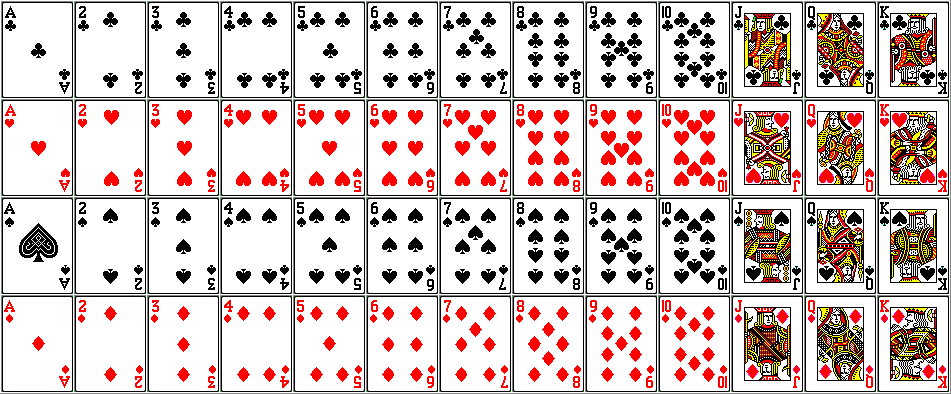
\includegraphics[width=0.8\textwidth]{playingcards}
\end{center}
\begin{example}[https://www.youtube.com/watch?v=h_RyIlkgV2M]{Drawing a card}
Suppose you draw one card from a standard 52-card deck. What is the probability of drawing an Ace?   \\

\marginnote{\bfseries Solution} There are 4 aces in a deck of cards. Let $A$ denote an event that the drawn card is an Ace. Then
\[  P(A) = \frac{4}{52}  = \frac{1}{13} \]
\end{example}

\begin{try}
When drawing a card from a standard 52-card deck, what is the probability of drawing a face card? \emph{Face cards include Jacks, Queens, and Kings}. What about the probability of drawing the King of Hearts?
\end{try}

\noindent Let's consider a more ``sweet'' example of calculating theoretical probabilities:
%%%%%%%%%%%%%%%%%%%%%%%%%%%%%%
\begin{example}[https://www.youtube.com/watch?v=7DSjUMJHnTk]{Cookies}
Lisa's cookie jar contains the following: 5 peanut butter, 10 oatmeal raisin, 12 chocolate chip, and 8 sugar cookies. If Lisa selects one cookie, what is the probability she gets a peanut butter cookie? \\

\marginnote{\bfseries  Solution \\ 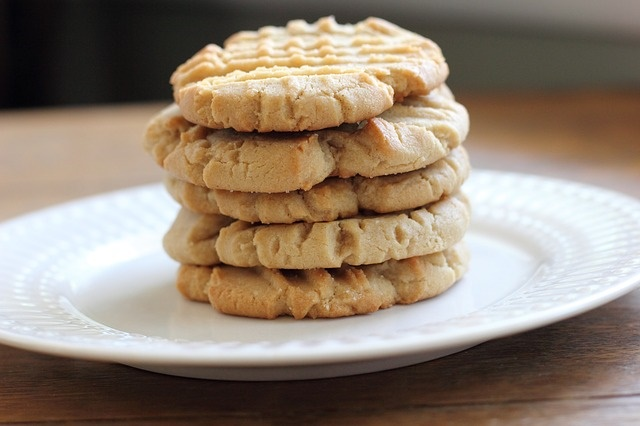
\includegraphics[height = .8in]{cookies}  } The total number of cookies in the jar is 35. Let $PB$ denote the event when a peanut butter cookie is selected, then
\[  P(PB) = \frac{5}{35} = \frac{1}{7} \]
\end{example}

\begin{try}
What is the probability that Lisa gets an oatmeal raisin cookie? What flavor of cookie is Lisa \emph{most likely} to get and why? 
\end{try} 
\vfill
\pagebreak

\subsection{Empirical Probability}
As long as we can list--or at least count--the sample space and the number of outcomes that correspond to our event, we can calculate basic probabilities by dividing, as we have done so far.  But there are many situations where this isn't feasible.  

For instance, take the example of a batter coming to the plate in a baseball game.  There's no way to even begin to list all the possible outcomes that could occur, much less count how many of them correspond to the batter getting a hit.  We'd still like to be able to estimate the likelihood of the batter getting a hit during this at-bat, though.  Just as sports fan do, then, we turn to this batter's previous performance; if he's gotten a hit in 200 of his last 1000 at-bats, we assume that the probability of a hit this time is $\frac{200}{1000}=0.200$.

Empirical probability is used when we observe the number of occurrences of an event. It is used to calculate probabilities based on the \emph{real data} that we observed and collected. To compute the empirical probability of an event $E$, denoted $P(E)$, we use the formula below:
\begin{formula}{Empirical probability}
\[  P(E) = \dfrac{\mbox{observed number of times $E$ occurs}}{\mbox{total number of observed occurrences}} \]
\end{formula} 

This can also be used to answer questions about sampling randomly from a population if we know the breakdown of the group.

\begin{example}[https://www.youtube.com/watch?v=_a7B5MAOXDg]{FCC students}
Consider the following information about FCC students' enrollment:

\begin{center}
\begin{tabular}{|c|c|}
\hline
Gender & Enrollment \\ \hline 
Female & 3653 \\ \hline
Male & 2580 \\ \hline 
\end{tabular}
\end{center}

If one person is randomly selected from all students at FCC, what is the probability of selecting a male?\\

\marginnote{\bfseries Solution} The total enrollment is 6233 students, thus we get:
\[  P(M) = \frac{2580}{6233} \approx 0.414 \]
\end{example} 

\begin{try}
Consider the following information about FCC students' enrollment:

\begin{center}
\begin{tabular}{|c|c|}
\hline
Status & Enrollment \\ \hline 
Full-time & 2359 \\ \hline
Part-time & 3874 \\ \hline 
\end{tabular}
\end{center}

If one person is randomly selected from the group, what is the probability of choosing a full-time student? Round your answer to 3 decimal places. 
\end{try} 

The next example contains a two-way table, often referred to as a \emph{contingency} table, which breaks down information about a group based on two criteria.  For example, the table below breaks down a group of 130 FCC students based on gender and which hand is their dominant hand:

\begin{center}
\begin{tabular}{|c|c|c|}
\hline
Gender & Right-handed & Left-handed \\ \hline 
Female & 58 & 13\\ \hline
Male & 47 & 12  \\ \hline
\end{tabular}
\end{center}

In order to use this to calculate probabilities if we randomly select someone from the group, we need to calculate totals for each category: the number of males, the number of females, the number of left-handed people, and the number of right-handed people.  This is done by simply summing each row and column; if we do that, we obtain the completed table below.

\begin{center}
\begin{tabular}{|c|c|c|c|}
\hline
Gender & Right-handed & Left-handed & \textbf{Total} \\ \hline 
Female & 58 & 13 & 71\\ \hline
Male & 47 & 12 & 59  \\ \hline
\textbf{Total} & 105 & 25 & 130 \\ \hline 
\end{tabular}
\end{center}

\begin{example}[https://www.youtube.com/watch?v=1aebOnTckVY]{FCC students}
Consider the following information about a group of 130 FCC students:

\begin{center}
\begin{tabular}{|c|c|c|c|}
\hline
Gender & Right-handed & Left-handed & \textbf{Total} \\ \hline 
Female & 58 & 13 & 71\\ \hline
Male & 47 & 12 & 59  \\ \hline
\textbf{Total} & 105 & 25 & 130 \\ \hline 
\end{tabular}
\end{center}

If one person is randomly selected from the group, what is the probability this student is left-handed? \\

\marginnote{\bfseries Solution} The total number of left-handed students in the group is 25, thus
\[  P(L) = \frac{25}{130} \approx 0.192 \]
\end{example}

\begin{try}
Using the table above, find the probability of selecting a female student. Round your final answer to three decimal places.
\end{try}

%%%%%%%%%%%%%%%%%%%%%%%%%%%%%%
\begin{example}[https://www.youtube.com/watch?v=odsxeO7wjqk]{Residency}
Consider the following information about students at Frederick Community College:

\begin{center}
\begin{tabular}{|c|c|}
\hline
Residence & Enrollment \\ \hline 
Frederick County & 5847\\ \hline
From another county in Maryland  & 245  \\ \hline 
Out of state & 141 \\ \hline
\end{tabular}
\end{center}

Each student can be assigned to one category only. If one person is randomly selected from the total group, what is the probability this student is from another county in Maryland?  \\

\marginnote{\bfseries Solution} Adding all the enrollments, we find that the total number of students is 6233, thus
\[  P(A) = \frac{245}{6233} \approx 0.039 \]
\end{example}

\begin{try}
Using the table above, find the probability of selecting an out-of-state student.  
\end{try}  
\vfill
\pagebreak

Now, let's go back to example 3: rolling a six-sided die and considering the event of rolling an odd number. If you were to roll the die only a few times, you might be
surprised if your observed results did not match the probability. If you were to roll the die a very large number of times, you
would expect that, overall, 1/2 of the rolls would result in an outcome of ``odd number.''  However, you would not expect exactly 1/2.  The long-term relative frequency of obtaining this result would approach the theoretical probability of 1/2 as the number of repetitions grows larger and larger. 

This important characteristic of probability experiments is known as the \textbf{Law of Large Numbers} which states that as the number of repetitions of an experiment is increased, the empirical probability obtained in the experiment tends to become closer and closer to the theoretical probability.

\begin{example}[https://www.youtube.com/watch?v=UbKc9wadf64]{Demonstrating the Law of Large Numbers}
Consider the following experiment: rolling a six-sided die 10 times, recording the outcomes and then taking the average. One can do this experiment by using a random number generator rather than physically rolling a die over and over again. Suppose the results are recorded in a table below: \\


\begin{center}
\begin{tabular}{|l|l|l|l|l|l|l|l|l|l|l|} \hline 
\textbf{Roll} & 1 & 2 & 3 & 4 & 5 & 6 & 7 & 8 & 9 & 10 \\ \hline
\textbf{Outcome} & 4 & 2 & 1 & 6 & 2 & 4 & 3 & 2 & 5 & 4 \\ \hline
\end{tabular}
\end{center}
We compute the average of the outcomes: 
\[  \dfrac{ 4 + 2 + 1 + 6 + 2 + 4 + 3 + 2 + 5 + 4}{10} = \frac{33}{10} = 3.3 \]

What will happen if we roll the die 100 times? 1000 times? 

\begin{center}
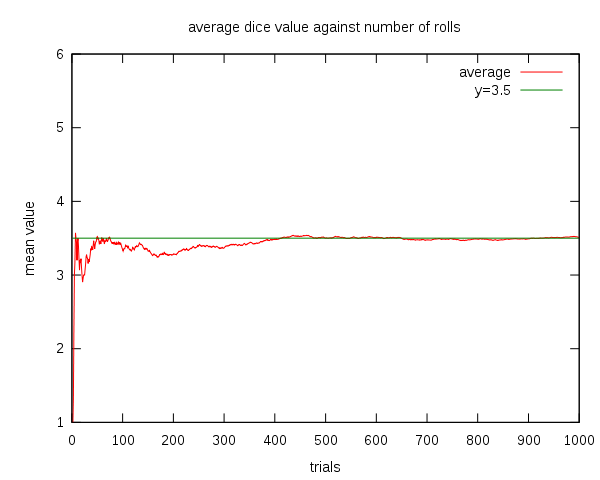
\includegraphics[scale=.5]{largenumbers}
\end{center}
You can see that as the number of rolls in this experiment increases, the average of the values of all the results approaches 3.5. If different people tried doing this experiment, their graphs would show a different shape over a small number of throws (at the left), but over a large number of rolls (to the right) they would be extremely similar.
\end{example}

\begin{exercises}

\pthree{A fair die is rolled. Find the probability of getting 4.}
\pthree{A fair die is rolled. Find the probability of getting less than 3.}
\pthree{A fair die is rolled. Find the probability of getting at least 5.}

\ptwo{You have a bag with 20 cherries, 14 sweet and 6 sour. If you pick a cherry at random, what is the probability that it will be sweet?}
\ptwo{A ball is drawn randomly from a jar that contains 6 red balls, 2 white balls, and 5 yellow balls. Find the probability of drawing a white ball.} 

\ptwo{Suppose you write each letter of the alphabet on a different slip of paper and put the slips into a hat. What is the probability of drawing one slip of paper from the hat at random and getting a consonant?}
\ptwo{In a survey, 205 people indicated they prefer cats, 160 indicated they prefer dogs, and 40 indicated they don't enjoy either pet. Find the probability that if a person is chosen at random, they prefer cats.}

\ptwo{A group of people were asked if they had run a red light in the last year. 150 responded ``yes'' and 185 responded ``no.'' Find the probability that if a person is chosen at random, they have run a red light in the last year.}
\ptwo{A U.S. roulette wheel has 38 pockets : 1 through 36, 0, and 00. 18 are black, 18 are red, and 2 are green. A play has a
dealer spin the wheel and a small ball in opposite directions. As the ball slows to stop, it can land with equal probability on 
the 38 slots. Find the probability of the ball landing on green.}

\pone{A glass jar contains 6 red, 5 green, 8 blue and 3 yellow marbles. If a single marble is
chosen at random from the jar, what is the probability of choosing
\begin{enumerate}[(a)]
\item a red marble?
\item a green marble?
\item a blue marble?
\end{enumerate}}

\pone { Lisa has a large bag of coins. After counting the coins, she recorded  the counts in the table below. She then decided to draw some coins at random, replacing each coin before the next draw.
	\begin{center}
	\begin{tabular}{ |c|c|c|c|}
	\hline
	Quarters & Nickels & Dimes & Pennies \\
	\hline 
	27 & 18 & 34 & 21   \\
	\hline	
	\end{tabular}
	\end{center}
	\begin{enumerate}[(a)]
		\item What is the probability that Lisa obtains a quarter on the first draw?
		\item What is the probability that Lisa obtains a penny or a dime on the second draw?
		\item What is the probability that Lisa obtains at most 10 cents worth of money on the third draw?
    \item What is the probability that Lisa does not get a nickel on the fourth draw?
  	\item What is the probability that Lisa obtains at least 10 cents worth of money on the fifth draw?
		\end{enumerate}}
		
\pone{Suppose you roll a pair of six-sided dice. 
\begin{enumerate}[(a)]
	\item List all possible outcomes of this experiment.
	\item What is the probability that the sum of the numbers on your dice is exactly 6?
	\item What is the probability that the sum of the numbers on your dice is at most 4?
	\item What is the probability that the sum of the numbers on your dice is at least 9?
\end{enumerate}}

\ptwo{I asked my Facebook friends to complete a two-question survey. They answered the following questions:
 Which beverage do you prefer in the morning: coffee or tea?  What is your gender? I summarized the results in following table:
\begin{center}
\begin{tabular}{|c|c|c|c|}
\hline
 & Coffee & Tea & \textbf{Total} \\
\hline
Female  & 37  & 24 & \textbf{61} \\
\hline
Male  & 22 & 31 & \textbf{53} \\
\hline
\textbf{Total }     & \textbf{59 }& \textbf{55} & \textbf{114} \\
\hline
\end{tabular}
\end{center}
\begin{enumerate}[(a)]
	\item What is the probability that I select a friend who prefers coffee?
	\item What is the probability that I select a friend who is female?
	\item What is the probability that I select a friend who is male and prefers tea?
	\vspace{.8in}
\end{enumerate}	}
\ptwo{A poll was taken of 14,056 working adults aged 40-70 to determine their level of
education. The participants were classified by sex and by level of education. The results
were as follows.
\begin{center}
\begin{tabular}{c|cc|c} \hline
Education Level     &  Male &  Female &  Total \\ \hline
High School or Less & 3141  &2434     &  5575  \\ 
Bachelor's Degree   & 3619  &3761     &  7380  \\
Master's Degree     & 534   &472      &  1006  \\
Ph.D.               & 52    &43       &  95    \\ \hline
Total 							& 7346  &6710     & 14,056 \\ 
\end{tabular}
\end{center}
A person is selected at random. Compute the following probabilities:
\begin{enumerate}[(a)]
	\item The probability that the selected person is a male
	\item The probability that the selected person does not have a Ph.D.
	\item The probability that the selected person has a Master's degree
	\item The probability that the selected person is female and has a  Master's degree
	\end{enumerate}	}
\end{exercises}


%%%%%%%%%%%%%%%%%%%%%%%%%%%%%%



